&%%
%% Emacs: Time-stamp: <2024-09-10 17:22:25 stefan>
%% VS Code: Last modified: 2024-09-05 10:56:58
%%
%% CV för aktuell användning i ansökan mot olika organisationer

\documentclass[a4paper,swedish,11pt]{article}

\usepackage[utf8]{inputenc}

% fet för rubriker
\usepackage{tgadventor}

%% visa geometrier

% brödtext
\usepackage[scaled=1.0]{gillius2}
\renewcommand*{\familydefault}{\sfdefault}

% specialfont för årtal
\usepackage{cinzel}
\usepackage[T1]{fontenc}    %% annars fungerar inte klipp-och-klistra från PDF självt

\usepackage{calc}
\usepackage{babel}
\usepackage[a4paper,headheight=39pt,top=3cm,bottom=2cm,left=1.5cm,right=1.5cm]{geometry}
\usepackage{fullminipage}
\usepackage{xcolor}
\usepackage{graphicx}
\usepackage[export]{adjustbox}
%% \usepackage{ragged2e}
\usepackage{enumitem}
\usepackage{blindtext}
\usepackage{adjustbox}
\usepackage[colorlinks=true, allcolors=blue]{hyperref}

\usepackage{fancyhdr}
\fancyhf[LH]{Stefan Skoglund\\Högalidsgatan 36\\521 61 Stenstorp}
\fancyhf[CH]{stefan.skoglund@agj.net\\%
  \href{http://www.linkedin.com/in/stefan-niskanen-skoglund-902aa0a1}{Linkedin:Stefan Skoglund}\\
  \href{https://github.com/Skaraborgfakir}{github: Skaraborgfakir}}
\fancyhf[RH]{0702--719 835}
\fancyhf[CF]{\href{https://skaraborgfakir.github.io/cv_generell_2024.pdf}{Länk till aktuell version}}
\pagestyle{fancy}

\newenvironment*{descriptioncv}[1]%
{%
  \textbf{\normalsize #1}%
  \begin{description}[nosep,font=\sffamily\bfseries, leftmargin=0.5cm,style=nextline]%
  }%
  {\end{description}\vspace{0.4cm}}
\newcommand*{\cvitem}[3]{\item[#1]{\cinzel\normalsize#2}\\#3}

% DEBUG:utmatning av uppgifter om storlekar,kerning osv
% \showoutput
\begin{document}
\begin{minipage}[t]{0.73\textwidth}
  \begin{descriptioncv}{Om mig själv} %% dela på utbildningar kompletta / kurser
  \item{Har ett intresse för att förstå en viss teknik inklusive att på ett pedagogiskt sätt
      presentera varför något är som det är.

      En liten dröm är att i framtiden i ett arbete inom signalprojektering få chansen att arbeta
      med ställverk 65 för att förstå hur konstruktörerna en gång i tiden tänkte. Jag har ganska så
      mycket tekniknostalgi.
    }
  \end{descriptioncv}

  \begin{descriptioncv}{Utbildningar} %% dela på utbildningar kompletta / kurser
    \cvitem{Stockholms tekniska institut}{Augusti 2022--Juni 2024}{STI:s YH-utbildning till järnvägsprojektör}
    \cvitem{Lexicon, Skaraborg}{Juni 2021-December 2021}{Utbildning i dotNet:programmering med JavaScript,C\#,
      HTML, CSS, Azure
      och Entity Framework med dess Identity server}
    \cvitem{YH:utbildning, Signaltekniker, Lärcenter i Falköping}{Augusti 2014--Juni 2015}{inriktning mot ERTMS,
      växlar, spårledningar vägskydd, ställverk 59 och kommunikation mellan EBISAT och DLC }
  \end{descriptioncv}

  \begin{descriptioncv}{Separata kurser} %% dela på utbildningar kompletta / kurser
    \cvitem{C, Umeås universitet}{Januari-- Mars 2022}{Programmering i C}
    \cvitem{Lexicon, Skaraborg}{December 2021}{AZ900:certifiering}
    \cvitem{Lexicon, Skaraborg}{Mars 2021}{Gått igenom Lexicons Test\&Bedömning för deras support- och
      dotNET-utbildningar}
    \cvitem{Historia A, Göteborgs universitet}{Januari-- Juni 2018}{A:grundkursen i historia}
    \cvitem{Historia B, Göteborgs universitet}{Augusti-- December 2018}{Fortsättningskurs i historia, I B:uppsatsen
      använder jag  en Umeåprästs livshistoria som en källa}
    \cvitem{Skriptprogrammering i Linux, Göteborgs universitet}{Våren 2019}{telemetri med \texttt{awk} och
      \texttt{bash}, del av ett mätteknikprogram vid Chalmers}
    \cvitem{Databasteknik A, Högskolan i Skövde}{2019}{grundläggande databaskonstruktion i MySQL}
    \cvitem{Datornätverk A, Högskolan i Skövde}{2019}{CISCO ICND1}
  \end{descriptioncv}
\end{minipage}%
\begin{minipage}[t]{0.24\textwidth}%
%%  \begin{description}[nosep]
    \raggedleft%
    \vspace{-\topskip+1cm}
    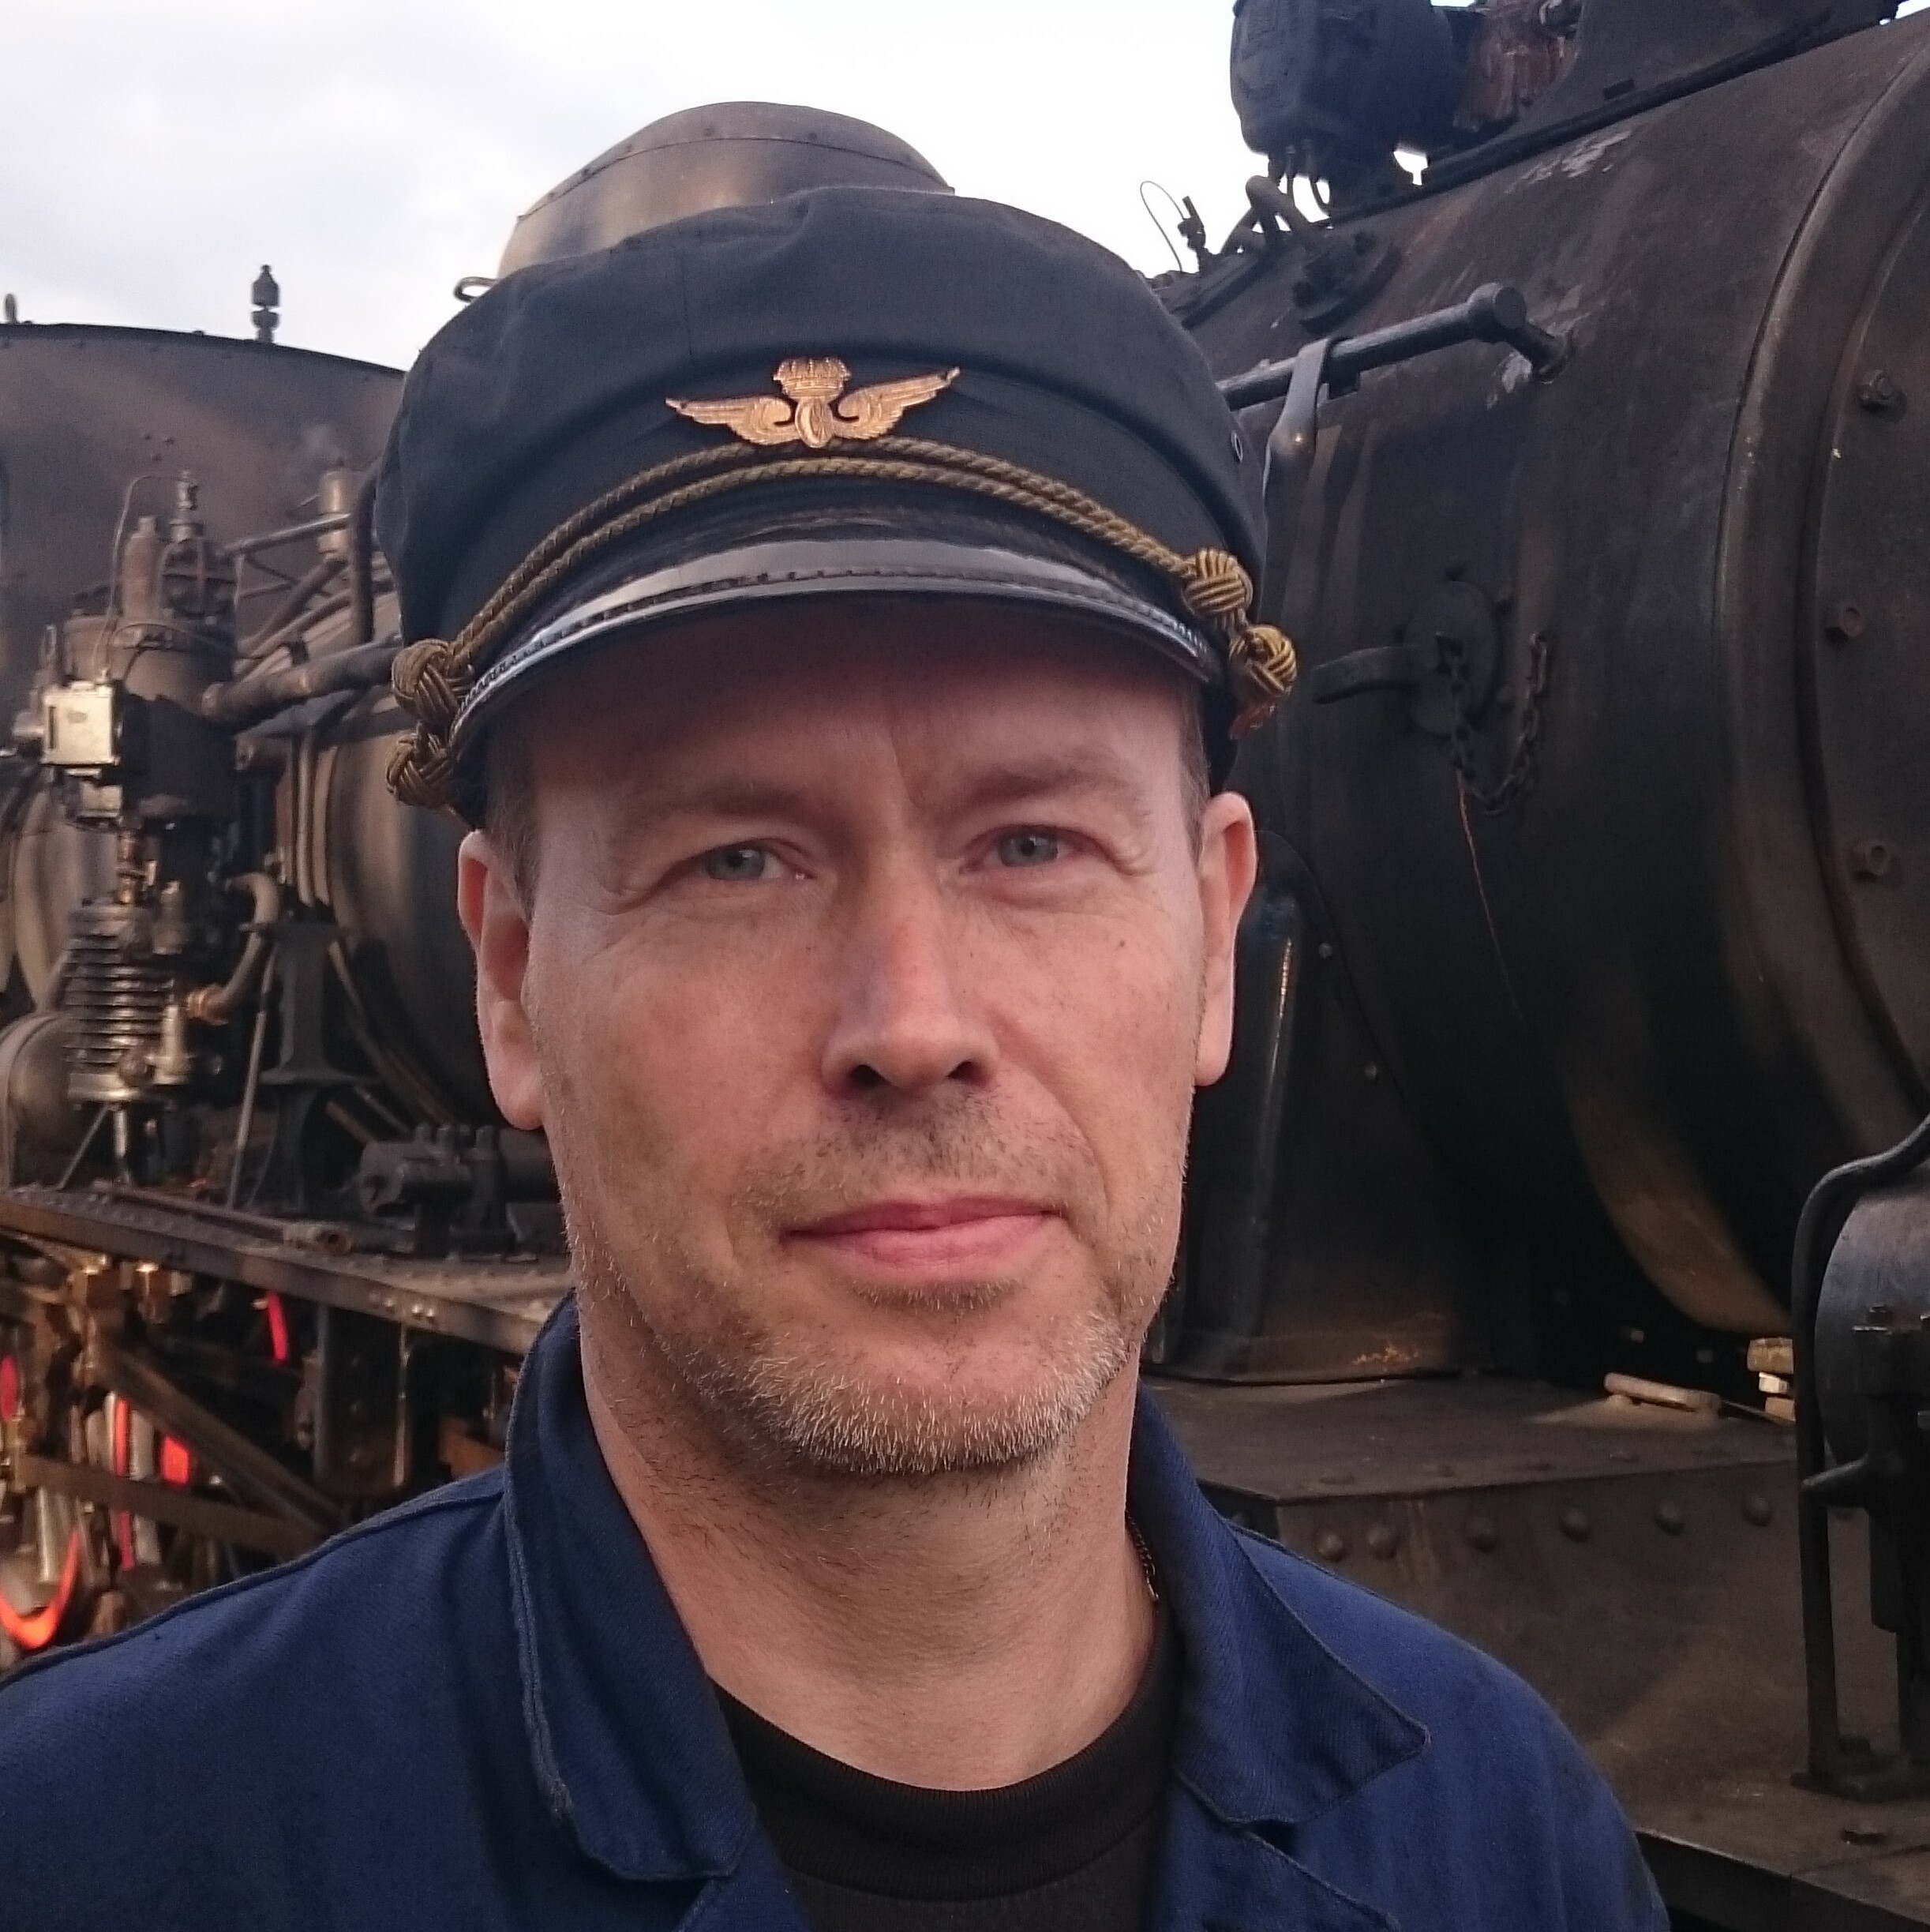
\includegraphics[height=3.5cm]{bild.jpg}

    %% \vspace{0.5cm}
    \textbf{Språk}
    \begin{description}[nosep,itemsep=0.1ex]
      \raggedleft\small%
    \item Svenska (modersmål)
    \item Engelska (van, samtal och skriftlig)
    \end{description}
\end{minipage}

\begin{minipage}[t]{0.73\textwidth}
  \begin{descriptioncv}{Separata kurser} %% dela på utbildningar kompletta / kurser
    \cvitem{Linux administration A, Högskolan i Skövde}{2014}{UNIX admin: epost med web:gränssnitt}
    \cvitem{UNIX B, Högskolan i Skövde}{2012}{UNIX admin: epost med web:gränssnitt}
    \cvitem{Modellering, Högskolan i Skövde}{2018}{UML med grupporienterad verksamhetsmodellering}
  \end{descriptioncv}

  \begin{descriptioncv}{Arbeten och praktikplatser}
    \cvitem{Projektör, Tyréns}{2023 Maj--Juli}{Praktik som projektör vid Tyréns kontor i Göteborg}
    \cvitem{Lärarevikarie, Falköpings kommun}{2022 Februari--}{Vikarie inom förskolan och grundskolan i Falköpings
      kommun}
    \cvitem{Signaltekniker, NVBS}{2017 Maj-- Augusti}{Uthyrd till INFRANORD för ny- och ombyggnads-arbeten i samband
      med att Citybanan i Stockholm skulle öppnas. Förberedelser för Getingmidjearbetena.}
    \cvitem{Signaltekniker, NVBS}{2016 Juli}{Uthyrd till INFRANORD som sommarvikarie till underhållet vid järnvägen
      i Stockhoolm.}
    \cvitem{Signaltekniker, NVBS}{2015 Juli-- Augusti}{Uthyrd som sommarvikarie till INFRANORDs underhållskontrakt
      vid centralstationen (Stockholm.)}
    \cvitem{Praktik, INFRANORD Herrljunga}{2015 Mars--Juni}{Praktik som signaltekniker vid underhållskontraktet
      i Herrljunga}
    \cvitem{Praktik, InfraTek Stockholm}{2014 Oktober}{Praktik som signaltekniker vid underhållskontraktet
      i Stockholm Nord/Hagalund}
    % \cvitem{Servicetekniker, Kronbergs hushållsservice, Skövde}{Mars 1996--November 2006}{reparation av
    %   vitvaror (spisar,tvättmaskiner och småapparater) och frånluftsvärmepumpar.
    %   Kundkontakt med planering av arbeten. Försäljning av ersättningsmaskiner. Justering
    %   av ventilationssystem.}
    % \cvitem{Telefonist, F6 Karlsborg}{1989-1990}{Miltex, flygvapnets radiosystem för kommunikation på flygbaser}
  \end{descriptioncv}

  \textbf{Examensarbetet}

  Mitt examensarbete vid STI omfattade tre frågor för MicroStation:
  \begin{itemize}
    \item Automatiserad provning av installationer av Microstation, specifikt att prova att utskrifter fungerar
      på ett förväntat sätt
    \item Centraliserad konfiguration av arbetsytor och ritningsuppsättningarna i dessa
    \item Automatiserad hantering av en användares licensnycklar för att kunna köra MicroStation i en miljö
      utan direktförbindelse via Internet med Bentley's licensieringstjänst dvs att nedhämtade nycklar ska
      distribueras inom ett internt nät till användarnas maskiner.
    \end{itemize}
    Detta medförde att jag fick lära mig systemadministration i Windows (använder CFEngine som ramverk.)
    Tester och prov skrivs i Powershell.
\end{minipage}

\begin{minipage}[t]{0.73\textwidth}
  \begin{descriptioncv}{Egna programmeringsprojekt}
    \cvitem{Automatisering av BIND}{2015--}{Automatiserad konfiguration av ISC:s BIND9:demon.
      Använder existerande JSON:beskrivningar av
      de olika systemen med namn, IP:adresser och vilka tjänster de har för att automatiskt generera DNS:zonbeskrivningar
      med kravet att löpnummer för zonen uppdateras på ett korrekt sätt.)}
    \cvitem{PKI:funktionalitet}{2014--}{Användning av publika certifikat med en struktur med fyra st
      certifikatutfärdare där de olika utfärdarna har olika ansvar.
      Rot-utfärdarens certifikat installeras på de system där det är nödvändigt.
      Mellannivåns certifikat är signerat av rot-diton medans dess funktion är en delegerad rotutfärdare
      men med korta löptider för dess eget certifikat.
      Applikations- och slutanvändare-certifikat hanteras av var sin specialiserad utfärdare.
      Paketet är skrivet för openssl och dess ''ca'':verktyg.}
    \cvitem{Automatisering av brandväggsregler}{2015--}{Automatiserad konfiguration av IPtable. Uppgifter om olika tjänster
      i nätet i JSON för att ange vilka avsändaradresser som är godkända för olika TCP:/UDP:portar. Acceptansför att
      kontrollera det genererade IPtable-skriptet exv inte blockerar SSH från egna maskiner. Gått igenom
      reglerna för ICMP för att ange och dokumentera varför viss trafik är nödvändig och OK eller om den är önskvärd.
      Samma typ av genomgång har gjorts för IPv6:trafik. Har via Hurricane Electric haft en globalt nåbar IPv6-adress
      i fem år jämfört med IP-onlys använding av Carrier-grade NAT.}
   \cvitem{IBM:s master the mainframe:program}{2021--}{har gått in i IBM:s master the mainframe:program
      för att lära mig den miljön (z/OS,COBOL,JCL). Ett resultat av mitt intresse för 1978:s års MVS}
  \end{descriptioncv}

  \textbf{Utvecklingstekniker}
  \begin{description}[nosep]
    %% \raggedleft\setlength\itemsep{0.1ex}\small%
    \small
  \item Objektorienterad programmering
  \item Människa-Maskin:interaktion
  \item UML
  \item C/C++
  \item Pascal
  \item Ada
  \item Python
  \end{description}

  \textbf{Linux/UNIX}
  \begin{description}[nosep,font=\sffamily\bfseries]
    %% \raggedleft\setlength\itemsep{0.1ex}
    \small%
  \item CFEngine (sedan 2012--)
  \item LINUX (RedHat 5 1997--)
  \item LINUX (Debian sedan 12 år)
  \item Solaris (SunOS4/SunOS5)
  \item PostgreSQL (för databaskurser)
  \item Datornätverk
  \end{description}

  \textbf{Andra IT:kunskaper}
  \begin{description}[nosep,itemsep=0.1ex]
  \item MS Word
  \item NetBSD
  \item MVS
  \item z/OS (deltar i IBM:s programmeringsevent \href{https://ibmzxplore.influitive.com/forum/}{IBM Z Xplore})
  \item \LaTeX
  \end{description}
\end{minipage}
\begin{minipage}[t]{0.24\textwidth}
  \vspace{22cm}
  \textbf{Colophon}
  \begin{description}[nosep,itemsep=0.1ex]
    \setlength\itemsep{0.1ex}\small%
    \raggedleft%
  \item Stefan Skoglund {\cinzel{2022}}
  \item Gillius
  \item Cinzel (årtal)
  \item \LaTeX%
  \end{description}%
\end{minipage}%
\end{document}
